\documentclass[10pt,a4paper]{article}
\usepackage[margin=0.65in]{geometry}
\usepackage{graphicx,booktabs,hyperref,amsmath,enumitem}
\usepackage[T1]{fontenc}
\usepackage{lmodern}
\input{outputs/metrics.tex}
\setlist{nosep}
\begin{document}
\begin{center}
{\Large\bfseries Momentum, Reversal, and Market States:\\[3pt]
A Modern-Sample Replication of Jegadeesh and Titman (1993)}\\[8pt]
Yufei Liu \quad Student ID: 3036759762 \quad ECO6067 Individual Project 04\\[3pt]
16 October 2026
\end{center}
\noindent\textbf{Abstract.}
This project revisits the winner-minus-loser strategy of Jegadeesh and Titman (1993) using course-supplied CRSP CIZ data. Tables I--III are reconstructed for 2002--2025, followed by a comparison with Kenneth French's Mom factor, reversal tests, a 36-month follow-up of six-month-ranked cohorts, and a market-state extension. The representative 6/6 spread is \MainSpread\% per month (HAC $t=\MainT$), while its CAPM alpha is \MainAlpha\% ($t=\AlphaT$). The different sample and data vintage prevent a literal reproduction of the original estimates.

\section{Research question and economic method}
The original paper asks whether relative strength predicts future stock returns and what this implies for market efficiency. A positive long-winner, short-loser return can reflect delayed adjustment to information, risk compensation, or temporary price pressure; portfolio returns alone do not identify a unique mechanism. The paper first establishes the pattern, then checks market beta, firm size, subgroups, and later return paths.

For each formation month, eligible NYSE and AMEX common stocks are ranked into deciles by their compounded returns over the preceding $J\in\{3,6,9,12\}$ months. P1 is the lowest-return decile and P10 the highest. Each cohort is held for $K\in\{3,6,9,12\}$ months; the month-$t$ portfolio averages the $K$ active, equal-weighted cohorts. Table I reports the P10--P1 spread for immediate formation and for a five-trading-observation gap. The latter approximates the original paper's one-week gap. Table II compares the post-ranking market beta and formation size of 6/6 deciles. Table III repeats 6/6 sorts within size and prior daily-beta groups and estimates market-model alphas.

The original study uses 1965--1989 NYSE/AMEX data; this project uses the supplied 2000--2025 CIZ source and reports 288 common months from January 2002 through December 2025. Market capitalization is retained in source units. No trading-cost or shorting-cost adjustment is applied.

\section{Statistical method and replication results}
Monthly mean returns are accompanied by Newey--West standard errors with $K-1$ lags to account for overlapping holdings. CAPM alpha is the intercept in a regression of portfolio excess return on value-weighted market excess return; for the zero-cost spread, the dependent variable is the spread itself. These HAC choices are transparent modern inference decisions and need not match every historical reported $t$ statistic.

\begin{table}[h]
\centering\small
\caption{Representative 6/6 findings, monthly percentage points where applicable}
\begin{tabular}{lrr}
\toprule
Measure & Original 1965--1989 & Modern 2002--2025\\
\midrule
P10--P1 raw mean & 0.950 ($t=3.07$) & \MainSpread\ ($t=\MainT$)\\
P10--P1 post-ranking beta & $-0.080$ & \BetaSpread\\
P10--P1 CAPM alpha & 1.000 ($t=3.23$) & \MainAlpha\ ($t=\AlphaT$)\\
\bottomrule
\end{tabular}
\end{table}

All 32 Table I modern-sample spread means are positive. The representative 6/6 raw estimate has a HAC $t$ below the usual two-sided 5\% threshold. Table II gives P1 beta \LoserBeta\ and P10 beta \WinnerBeta; their negative difference means a simple positive market-beta premium cannot explain the positive long-short mean. The all-stock Table III alpha is positive, and spreads are larger among small and high-prior-beta stocks. Differences between subgroup spreads are descriptive because this report does not test them directly. Complete decile cells and joint HAC Wald tests are in \texttt{outputs/tables/}.

\section{Extension 1: constructed momentum versus French Mom}
The project builds a separate six-cell, value-weighted factor from NYSE size and momentum breakpoints. Its signal uses months $t-12$ through $t-2$, omitting $t-1$. The constructed factor is one-half of Small High plus Big High minus one-half of Small Low plus Big Low. Over 288 common months, its correlation with the public French US Mom factor is \MomCorrelation, and monthly tracking error is \MomTrackingError\ percentage points. This close match supports the implementation, while differences in source vintage and eligibility remain. The official Mom design differs from the equal-weighted, overlapping deciles in Tables I--III.

\begin{figure}[h]
\centering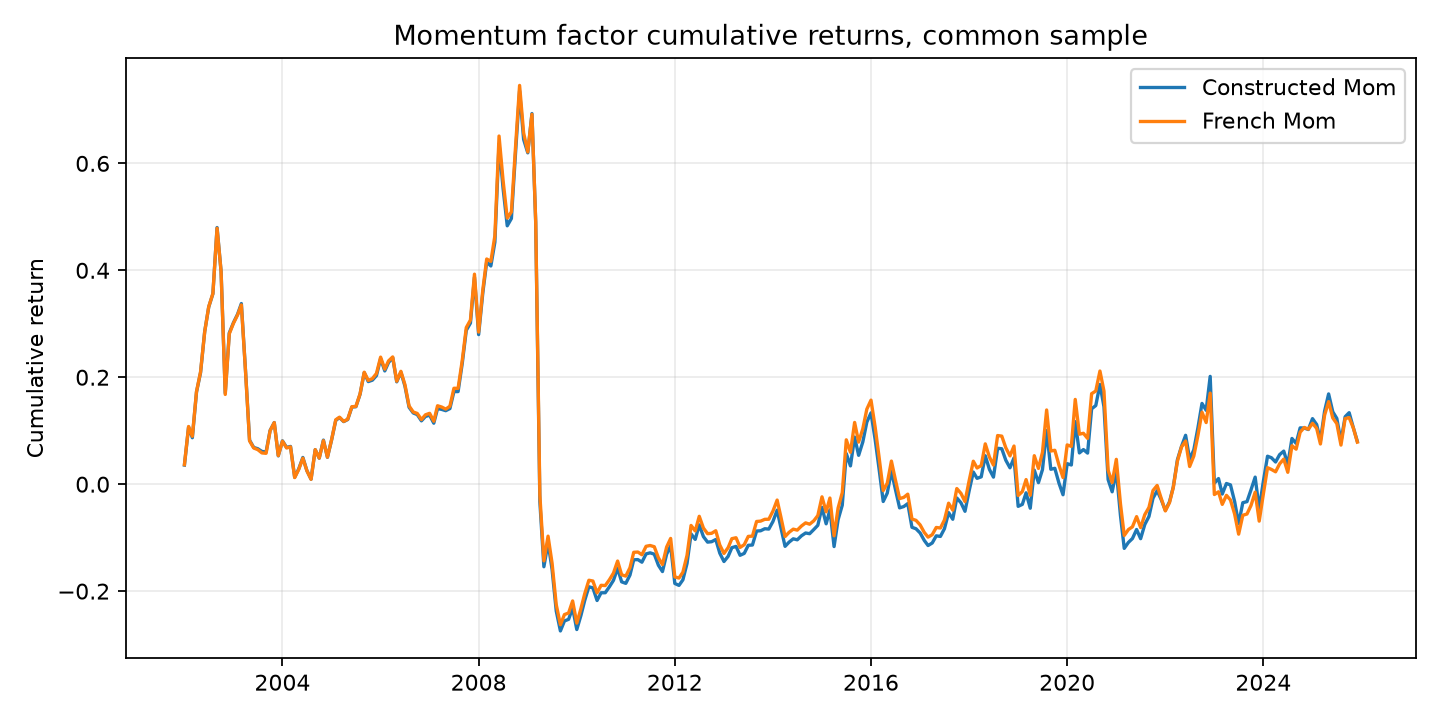
\includegraphics[width=.72\linewidth]{outputs/figures/extension_mom_cumulative.png}
\caption{Constructed and public Mom cumulative paths.}
\end{figure}

\section{Extension 2: reversal and event-time follow-up}
One-month reversal ranks the prior month's returns and holds P1--P10 for the next month. Its mean is \ShortReversal\% per month; the HAC $t$ is 1.07. For long-run reversal, seven nonoverlapping three-year cohorts are ranked on 36-month market-adjusted returns. Their cumulative P1--P10 spread at 36 months is \LongReversal\ percentage points. Seven cohorts give limited precision, and this is an extension inspired by De Bondt and Thaler (1985), not their literal portfolio construction.

A distinct analysis freezes the winners and losers selected on six-month returns and follows those \emph{same} cohorts for 36 months. The mean cumulative P10--P1 spread is \EventTwelve\ percentage points at month 12 and \EventThirtySix\ points at month 36. HAC intervals at both horizons include zero. This asks a question closer to the original paper's Table VII than the separate 36/36 reversal strategy, but cannot establish a later reversal in this sample.

\begin{figure}[h]
\centering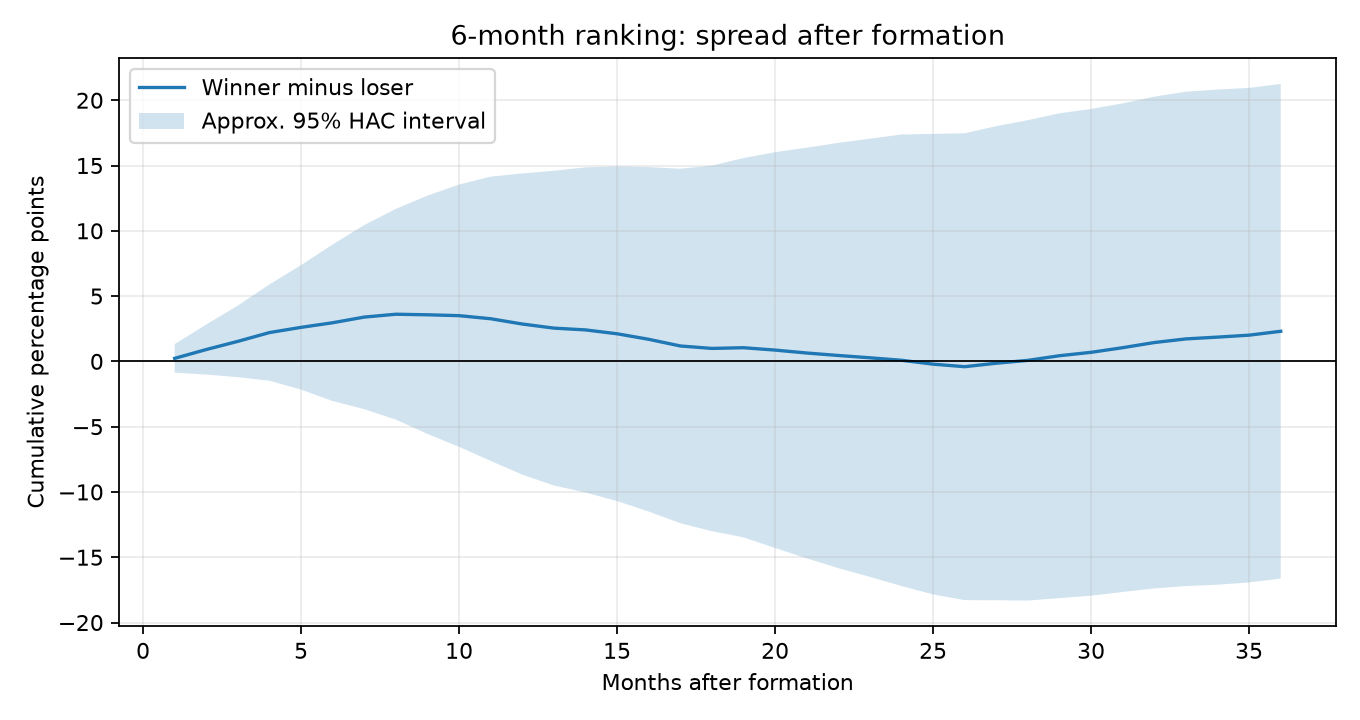
\includegraphics[width=.60\linewidth]{outputs/figures/event_time_6m_path.png}
\caption{Event-time path after six-month momentum ranking.}
\end{figure}

\noindent\textit{Reading the reversal evidence.}
These three tests answer different questions. The one-month sort checks whether last month's ranking reverses immediately; its positive loser-minus-winner mean has a modest HAC statistic and does not establish a reliable short-run premium. The 36/36 sort asks whether stocks with weak returns over three years subsequently outperform strong performers. Its 36-month cumulative spread is positive, but only seven nonoverlapping cohorts contribute, so a few market episodes can strongly affect the estimate. The event-time path instead follows stocks selected by the original six-month momentum signal. Its cumulative spread changes little between months 12 and 36 in this sample, and the intervals at both horizons include zero. These results therefore do not show a statistically clear decay or reversal of the original momentum portfolios. Later event months also average only stocks with available returns, so changes in portfolio composition can affect the path.

\clearpage
\section{Extension 3: momentum across prior market states}
The 6/6 Table I spread is classified by the sign of the market's compounded return over the prior 12 complete months, which is observable before the test month. Mean momentum return is \StateUp\% after a nonnegative prior-year market return and \StateDown\% after a negative one. The down-minus-nonnegative difference is \StateDifference\ percentage points per month, with HAC two-sided $p=\StateP$. Its 95\% interval includes zero. An especially poor month, April 2009, influences the difference. The same-month rebound split is descriptive and cannot be used as an advance trading signal.

\begin{figure}[h]
\centering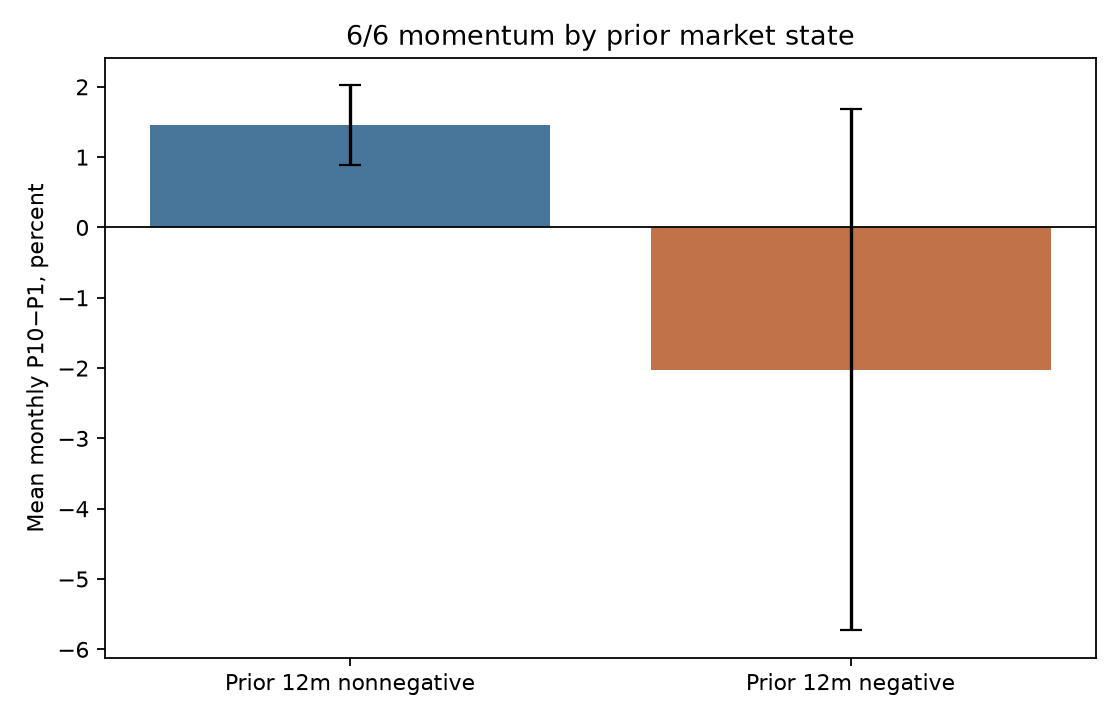
\includegraphics[width=.72\linewidth]{outputs/figures/extension_market_state.png}
\caption{Six-month momentum returns by prior 12-month market state.}
\end{figure}

\section{Interpretation, limits, and reproducibility}
The positive modern mean and negative winner-minus-loser beta resemble the original qualitative pattern, but the modern raw 6/6 mean is less precisely estimated. The sample period, CIZ return conventions, stock eligibility, five-observation gap, and HAC inference limit numerical comparisons with the historical paper. Market-model alpha depends on the chosen risk model. Neither the sorts nor the market-state comparison identify a causal behavioral mechanism or a net implementable trading profit.

Run \texttt{python3 code/run\_all.py} from the repository root with the course's licensed files installed as described in \texttt{data/raw/README.md}. This regenerates the tables, figures, reports, and this PDF. The source CSVs are excluded from the public repository. The full AI-use statement is in \texttt{AI\_USE\_DISCLOSURE.md}; detailed implementation and validation notes are in \texttt{reports/}.

\begin{thebibliography}{9}\footnotesize
\bibitem{jt} Jegadeesh, N., and S. Titman (1993). Returns to Buying Winners and Selling Losers: Implications for Stock Market Efficiency. \emph{Journal of Finance} 48(1), 65--91.
\bibitem{j90} Jegadeesh, N. (1990). Evidence of Predictable Behavior of Security Returns. \emph{Journal of Finance} 45(3), 881--898.
\bibitem{dbt} De Bondt, W. F. M., and R. Thaler (1985). Does the Stock Market Overreact? \emph{Journal of Finance} 40(3), 793--805.
\bibitem{dm} Daniel, K., and T. Moskowitz (2016). Momentum Crashes. \emph{Journal of Financial Economics} 122(2), 221--247.
\bibitem{french} Kenneth R. French Data Library. US Momentum Factor, public monthly series and construction notes.
\end{thebibliography}
\end{document}
